\documentclass[]{article}
\usepackage{lmodern}
\usepackage{amssymb,amsmath}
\usepackage{ifxetex,ifluatex}
\usepackage{fixltx2e} % provides \textsubscript
\ifnum 0\ifxetex 1\fi\ifluatex 1\fi=0 % if pdftex
  \usepackage[T1]{fontenc}
  \usepackage[utf8]{inputenc}
\else % if luatex or xelatex
  \ifxetex
    \usepackage{mathspec}
  \else
    \usepackage{fontspec}
  \fi
  \defaultfontfeatures{Ligatures=TeX,Scale=MatchLowercase}
\fi
% use upquote if available, for straight quotes in verbatim environments
\IfFileExists{upquote.sty}{\usepackage{upquote}}{}
% use microtype if available
\IfFileExists{microtype.sty}{%
\usepackage{microtype}
\UseMicrotypeSet[protrusion]{basicmath} % disable protrusion for tt fonts
}{}
\usepackage[margin=2.54cm]{geometry}
\usepackage{hyperref}
\hypersetup{unicode=true,
            pdftitle={Assignment 7: High Frequency Data},
            pdfauthor={Jake Greif},
            pdfborder={0 0 0},
            breaklinks=true}
\urlstyle{same}  % don't use monospace font for urls
\usepackage{color}
\usepackage{fancyvrb}
\newcommand{\VerbBar}{|}
\newcommand{\VERB}{\Verb[commandchars=\\\{\}]}
\DefineVerbatimEnvironment{Highlighting}{Verbatim}{commandchars=\\\{\}}
% Add ',fontsize=\small' for more characters per line
\usepackage{framed}
\definecolor{shadecolor}{RGB}{248,248,248}
\newenvironment{Shaded}{\begin{snugshade}}{\end{snugshade}}
\newcommand{\AlertTok}[1]{\textcolor[rgb]{0.94,0.16,0.16}{#1}}
\newcommand{\AnnotationTok}[1]{\textcolor[rgb]{0.56,0.35,0.01}{\textbf{\textit{#1}}}}
\newcommand{\AttributeTok}[1]{\textcolor[rgb]{0.77,0.63,0.00}{#1}}
\newcommand{\BaseNTok}[1]{\textcolor[rgb]{0.00,0.00,0.81}{#1}}
\newcommand{\BuiltInTok}[1]{#1}
\newcommand{\CharTok}[1]{\textcolor[rgb]{0.31,0.60,0.02}{#1}}
\newcommand{\CommentTok}[1]{\textcolor[rgb]{0.56,0.35,0.01}{\textit{#1}}}
\newcommand{\CommentVarTok}[1]{\textcolor[rgb]{0.56,0.35,0.01}{\textbf{\textit{#1}}}}
\newcommand{\ConstantTok}[1]{\textcolor[rgb]{0.00,0.00,0.00}{#1}}
\newcommand{\ControlFlowTok}[1]{\textcolor[rgb]{0.13,0.29,0.53}{\textbf{#1}}}
\newcommand{\DataTypeTok}[1]{\textcolor[rgb]{0.13,0.29,0.53}{#1}}
\newcommand{\DecValTok}[1]{\textcolor[rgb]{0.00,0.00,0.81}{#1}}
\newcommand{\DocumentationTok}[1]{\textcolor[rgb]{0.56,0.35,0.01}{\textbf{\textit{#1}}}}
\newcommand{\ErrorTok}[1]{\textcolor[rgb]{0.64,0.00,0.00}{\textbf{#1}}}
\newcommand{\ExtensionTok}[1]{#1}
\newcommand{\FloatTok}[1]{\textcolor[rgb]{0.00,0.00,0.81}{#1}}
\newcommand{\FunctionTok}[1]{\textcolor[rgb]{0.00,0.00,0.00}{#1}}
\newcommand{\ImportTok}[1]{#1}
\newcommand{\InformationTok}[1]{\textcolor[rgb]{0.56,0.35,0.01}{\textbf{\textit{#1}}}}
\newcommand{\KeywordTok}[1]{\textcolor[rgb]{0.13,0.29,0.53}{\textbf{#1}}}
\newcommand{\NormalTok}[1]{#1}
\newcommand{\OperatorTok}[1]{\textcolor[rgb]{0.81,0.36,0.00}{\textbf{#1}}}
\newcommand{\OtherTok}[1]{\textcolor[rgb]{0.56,0.35,0.01}{#1}}
\newcommand{\PreprocessorTok}[1]{\textcolor[rgb]{0.56,0.35,0.01}{\textit{#1}}}
\newcommand{\RegionMarkerTok}[1]{#1}
\newcommand{\SpecialCharTok}[1]{\textcolor[rgb]{0.00,0.00,0.00}{#1}}
\newcommand{\SpecialStringTok}[1]{\textcolor[rgb]{0.31,0.60,0.02}{#1}}
\newcommand{\StringTok}[1]{\textcolor[rgb]{0.31,0.60,0.02}{#1}}
\newcommand{\VariableTok}[1]{\textcolor[rgb]{0.00,0.00,0.00}{#1}}
\newcommand{\VerbatimStringTok}[1]{\textcolor[rgb]{0.31,0.60,0.02}{#1}}
\newcommand{\WarningTok}[1]{\textcolor[rgb]{0.56,0.35,0.01}{\textbf{\textit{#1}}}}
\usepackage{graphicx,grffile}
\makeatletter
\def\maxwidth{\ifdim\Gin@nat@width>\linewidth\linewidth\else\Gin@nat@width\fi}
\def\maxheight{\ifdim\Gin@nat@height>\textheight\textheight\else\Gin@nat@height\fi}
\makeatother
% Scale images if necessary, so that they will not overflow the page
% margins by default, and it is still possible to overwrite the defaults
% using explicit options in \includegraphics[width, height, ...]{}
\setkeys{Gin}{width=\maxwidth,height=\maxheight,keepaspectratio}
\IfFileExists{parskip.sty}{%
\usepackage{parskip}
}{% else
\setlength{\parindent}{0pt}
\setlength{\parskip}{6pt plus 2pt minus 1pt}
}
\setlength{\emergencystretch}{3em}  % prevent overfull lines
\providecommand{\tightlist}{%
  \setlength{\itemsep}{0pt}\setlength{\parskip}{0pt}}
\setcounter{secnumdepth}{0}
% Redefines (sub)paragraphs to behave more like sections
\ifx\paragraph\undefined\else
\let\oldparagraph\paragraph
\renewcommand{\paragraph}[1]{\oldparagraph{#1}\mbox{}}
\fi
\ifx\subparagraph\undefined\else
\let\oldsubparagraph\subparagraph
\renewcommand{\subparagraph}[1]{\oldsubparagraph{#1}\mbox{}}
\fi

%%% Use protect on footnotes to avoid problems with footnotes in titles
\let\rmarkdownfootnote\footnote%
\def\footnote{\protect\rmarkdownfootnote}

%%% Change title format to be more compact
\usepackage{titling}

% Create subtitle command for use in maketitle
\providecommand{\subtitle}[1]{
  \posttitle{
    \begin{center}\large#1\end{center}
    }
}

\setlength{\droptitle}{-2em}

  \title{Assignment 7: High Frequency Data}
    \pretitle{\vspace{\droptitle}\centering\huge}
  \posttitle{\par}
    \author{Jake Greif}
    \preauthor{\centering\large\emph}
  \postauthor{\par}
    \date{}
    \predate{}\postdate{}
  

\begin{document}
\maketitle

\hypertarget{overview}{%
\subsection{OVERVIEW}\label{overview}}

This exercise accompanies the lessons in Hydrologic Data Analysis on
high frequency data

\hypertarget{directions}{%
\subsection{Directions}\label{directions}}

\begin{enumerate}
\def\labelenumi{\arabic{enumi}.}
\tightlist
\item
  Change ``Student Name'' on line 3 (above) with your name.
\item
  Work through the steps, \textbf{creating code and output} that fulfill
  each instruction.
\item
  Be sure to \textbf{answer the questions} in this assignment document.
\item
  When you have completed the assignment, \textbf{Knit} the text and
  code into a single pdf file.
\item
  After Knitting, submit the completed exercise (pdf file) to the
  dropbox in Sakai. Add your last name into the file name (e.g.,
  ``A07\_Chamberlin.pdf'') prior to submission.
\end{enumerate}

The completed exercise is due on 16 October 2019 at 9:00 am.

\hypertarget{setup}{%
\subsection{Setup}\label{setup}}

\begin{enumerate}
\def\labelenumi{\arabic{enumi}.}
\tightlist
\item
  Verify your working directory is set to the R project file,
\item
  Load the StreamPULSE, streamMetabolizer and tidyverse packages.
\item
  Set your ggplot theme (can be theme\_classic or something else)
\end{enumerate}

\begin{Shaded}
\begin{Highlighting}[]
\KeywordTok{getwd}\NormalTok{()}
\end{Highlighting}
\end{Shaded}

\begin{verbatim}
## [1] "/Users/jakegreif/Duke/Fall_2019/Hydrologic_Data_Analysis"
\end{verbatim}

\begin{Shaded}
\begin{Highlighting}[]
\KeywordTok{library}\NormalTok{(tidyverse)}
\end{Highlighting}
\end{Shaded}

\begin{verbatim}
## -- Attaching packages ------------------------------------------------------------------ tidyverse 1.2.1 --
\end{verbatim}

\begin{verbatim}
## v ggplot2 3.2.1     v purrr   0.3.2
## v tibble  2.1.3     v dplyr   0.8.3
## v tidyr   1.0.0     v stringr 1.4.0
## v readr   1.3.1     v forcats 0.4.0
\end{verbatim}

\begin{verbatim}
## -- Conflicts --------------------------------------------------------------------- tidyverse_conflicts() --
## x dplyr::filter() masks stats::filter()
## x dplyr::lag()    masks stats::lag()
\end{verbatim}

\begin{Shaded}
\begin{Highlighting}[]
\KeywordTok{library}\NormalTok{(StreamPULSE)}
\end{Highlighting}
\end{Shaded}

\begin{verbatim}
## Loading required package: shiny
\end{verbatim}

\begin{verbatim}
## Loading required package: Cairo
\end{verbatim}

\begin{Shaded}
\begin{Highlighting}[]
\KeywordTok{library}\NormalTok{(streamMetabolizer)}
\end{Highlighting}
\end{Shaded}

\begin{verbatim}
## USGS Active Research Package:
## https://owi.usgs.gov/R/packages.html#research
\end{verbatim}

\begin{verbatim}
## This package is in development. We are using it for our own
## applications and welcome flexible, resilient users who can help us
## make the package better. Details of the user interface and model
## implementations will change. Please give us feedback at
## https://github.com/USGS-R/streamMetabolizer/issues/new.
\end{verbatim}

\begin{verbatim}
## Can't check GitHub for new package versions just now. We'll try again next time.
\end{verbatim}

\begin{Shaded}
\begin{Highlighting}[]
\KeywordTok{library}\NormalTok{(EcoHydRology)}
\end{Highlighting}
\end{Shaded}

\begin{verbatim}
## Loading required package: operators
\end{verbatim}

\begin{verbatim}
## 
## Attaching package: 'operators'
\end{verbatim}

\begin{verbatim}
## The following object is masked from 'package:forcats':
## 
##     %>%
\end{verbatim}

\begin{verbatim}
## The following object is masked from 'package:stringr':
## 
##     %>%
\end{verbatim}

\begin{verbatim}
## The following object is masked from 'package:dplyr':
## 
##     %>%
\end{verbatim}

\begin{verbatim}
## The following object is masked from 'package:purrr':
## 
##     %>%
\end{verbatim}

\begin{verbatim}
## The following object is masked from 'package:tidyr':
## 
##     %>%
\end{verbatim}

\begin{verbatim}
## The following objects are masked from 'package:base':
## 
##     options, strrep
\end{verbatim}

\begin{verbatim}
## Loading required package: topmodel
\end{verbatim}

\begin{verbatim}
## Loading required package: DEoptim
\end{verbatim}

\begin{verbatim}
## Loading required package: parallel
\end{verbatim}

\begin{verbatim}
## 
## DEoptim package
## Differential Evolution algorithm in R
## Authors: D. Ardia, K. Mullen, B. Peterson and J. Ulrich
\end{verbatim}

\begin{verbatim}
## Loading required package: XML
\end{verbatim}

\begin{Shaded}
\begin{Highlighting}[]
\KeywordTok{library}\NormalTok{(xts)}
\end{Highlighting}
\end{Shaded}

\begin{verbatim}
## Loading required package: zoo
\end{verbatim}

\begin{verbatim}
## 
## Attaching package: 'zoo'
\end{verbatim}

\begin{verbatim}
## The following objects are masked from 'package:base':
## 
##     as.Date, as.Date.numeric
\end{verbatim}

\begin{verbatim}
## Registered S3 method overwritten by 'xts':
##   method     from
##   as.zoo.xts zoo
\end{verbatim}

\begin{verbatim}
## 
## Attaching package: 'xts'
\end{verbatim}

\begin{verbatim}
## The following objects are masked from 'package:dplyr':
## 
##     first, last
\end{verbatim}

\begin{Shaded}
\begin{Highlighting}[]
\KeywordTok{library}\NormalTok{(dygraphs)}
\end{Highlighting}
\end{Shaded}

\begin{verbatim}
## This version of Shiny is designed to work with 'htmlwidgets' >= 1.5.
##     Please upgrade via install.packages('htmlwidgets').
\end{verbatim}

\begin{verbatim}
## 
## Attaching package: 'dygraphs'
\end{verbatim}

\begin{verbatim}
## The following object is masked from 'package:operators':
## 
##     %>%
\end{verbatim}

\begin{Shaded}
\begin{Highlighting}[]
\KeywordTok{theme_set}\NormalTok{(}\KeywordTok{theme_classic}\NormalTok{())}
\end{Highlighting}
\end{Shaded}

\begin{enumerate}
\def\labelenumi{\arabic{enumi}.}
\setcounter{enumi}{3}
\item
  Download data from the Stream Pulse portal using
  \texttt{request\_data()} for the Kansas River, (``KS\_KANSASR'').
  Download the discharge (\texttt{Discharge\_m3s}), disolved oxygen
  (\texttt{DO\_mgL}) and nitrate data (\texttt{Nitrate\_mgL}) for the
  entire period of record
\item
  Reformat the data into one dataframe with columns DateTime\_UTC,
  DateTime\_Solar (using \texttt{convert\_UTC\_to\_solartime()}),
  SiteName, DO\_mgL, Discharge\_m3s, and Nitrate\_mgL.
\end{enumerate}

\begin{Shaded}
\begin{Highlighting}[]
\NormalTok{KSdat <-}\StringTok{ }\KeywordTok{request_data}\NormalTok{(}
  \DataTypeTok{sitecode =} \StringTok{"KS_KANSASR"}\NormalTok{,}
  \DataTypeTok{variables =} \KeywordTok{c}\NormalTok{(}\StringTok{'DO_mgL'}\NormalTok{, }\StringTok{'Discharge_m3s'}\NormalTok{, }\StringTok{'Nitrate_mgL'}\NormalTok{))}
\end{Highlighting}
\end{Shaded}

\begin{verbatim}
## You may omit the "variables" parameter to automatically retrieve
##  all variables necessary for metabolism modeling.
\end{verbatim}

\begin{verbatim}
## 
## API call: https://data.streampulse.org/api?sitecode=KS_KANSASR&variables=DO_mgL,Discharge_m3s,Nitrate_mgL&flags=true
## 
## Retrieved the following variables:
##   DO_mgL, Discharge_m3s, Nitrate_mgL
\end{verbatim}

\begin{Shaded}
\begin{Highlighting}[]
\NormalTok{KS.lon <-}\StringTok{ }\NormalTok{KSdat[[}\DecValTok{2}\NormalTok{]]}\OperatorTok{$}\NormalTok{lon}

\NormalTok{KSdat.df <-}\StringTok{ }\NormalTok{KSdat[[}\DecValTok{1}\NormalTok{]] }\OperatorTok
\StringTok{  }\KeywordTok{spread}\NormalTok{(}\DataTypeTok{value =}\NormalTok{ value, }\DataTypeTok{key =}\NormalTok{ variable) }\OperatorTok
\StringTok{  }\KeywordTok{mutate}\NormalTok{(}\DataTypeTok{DateTime_Solar =} \KeywordTok{convert_UTC_to_solartime}\NormalTok{(DateTime_UTC, KS.lon))}

\NormalTok{KSdat.df <-}\StringTok{ }\KeywordTok{select}\NormalTok{(KSdat.df, }\KeywordTok{c}\NormalTok{(}\OperatorTok{-}\NormalTok{flagtype, }\OperatorTok{-}\NormalTok{flagcomment))}
\end{Highlighting}
\end{Shaded}

\begin{enumerate}
\def\labelenumi{\arabic{enumi}.}
\setcounter{enumi}{5}
\tightlist
\item
  Plot each of the 3 variables against solar time for the period of
  record
\end{enumerate}

\begin{Shaded}
\begin{Highlighting}[]
\KeywordTok{ggplot}\NormalTok{(KSdat.df, }\KeywordTok{aes}\NormalTok{(}\DataTypeTok{x =}\NormalTok{ DateTime_Solar, }\DataTypeTok{y =}\NormalTok{ Discharge_m3s)) }\OperatorTok{+}\StringTok{ }\KeywordTok{geom_line}\NormalTok{()}
\end{Highlighting}
\end{Shaded}

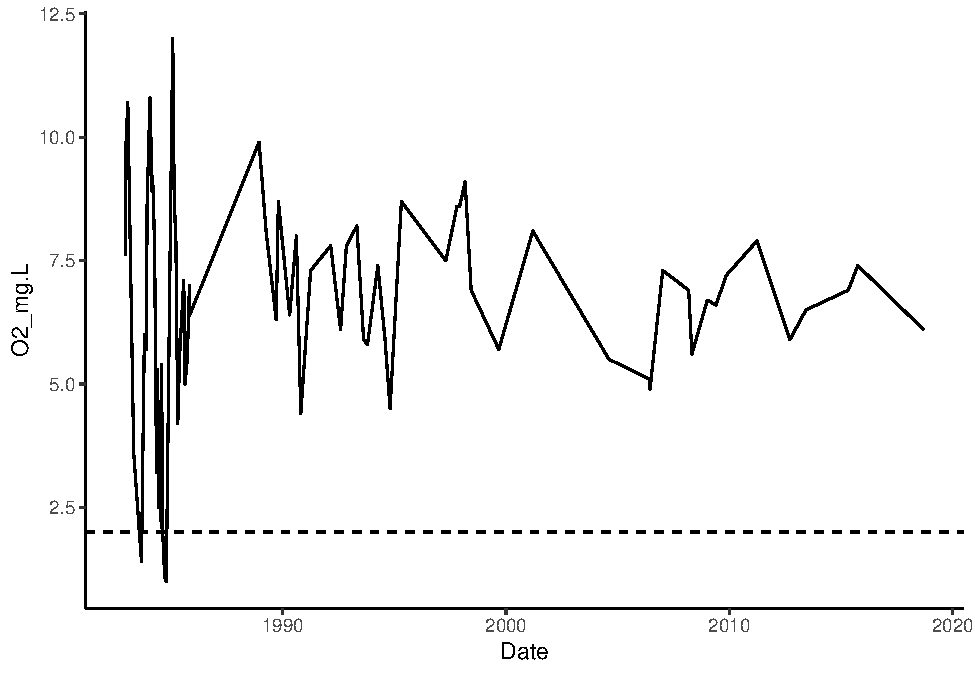
\includegraphics{A07_HighFrequencyData_files/figure-latex/unnamed-chunk-1-1.pdf}

\begin{Shaded}
\begin{Highlighting}[]
\KeywordTok{ggplot}\NormalTok{(KSdat.df, }\KeywordTok{aes}\NormalTok{(}\DataTypeTok{x =}\NormalTok{ DateTime_Solar, }\DataTypeTok{y =}\NormalTok{ DO_mgL)) }\OperatorTok{+}\StringTok{ }\KeywordTok{geom_line}\NormalTok{()}
\end{Highlighting}
\end{Shaded}

\includegraphics{A07_HighFrequencyData_files/figure-latex/unnamed-chunk-1-2.pdf}

\begin{Shaded}
\begin{Highlighting}[]
\KeywordTok{ggplot}\NormalTok{(KSdat.df, }\KeywordTok{aes}\NormalTok{(}\DataTypeTok{x =}\NormalTok{ DateTime_Solar, }\DataTypeTok{y =}\NormalTok{ Nitrate_mgL)) }\OperatorTok{+}\StringTok{ }\KeywordTok{geom_line}\NormalTok{()}
\end{Highlighting}
\end{Shaded}

\includegraphics{A07_HighFrequencyData_files/figure-latex/unnamed-chunk-1-3.pdf}

\begin{enumerate}
\def\labelenumi{\arabic{enumi}.}
\setcounter{enumi}{6}
\tightlist
\item
  How will you address gaps in these dataseries?
\end{enumerate}

\begin{quote}
I will remove the NAs first, and then check the the gaps in the data. If
the gaps are less than 12 hours, I'll ignore them because the data spans
several month.
\end{quote}

\begin{enumerate}
\def\labelenumi{\arabic{enumi}.}
\setcounter{enumi}{7}
\tightlist
\item
  How does the daily amplitude of oxygen concentration swings change
  over the season? What might cause this?
\end{enumerate}

\begin{quote}
The amplitude of daily DO increases as the seasons change from winter to
summer. This is likely due to the increased biological activity (and
therefore respiration and photosynthesis) in the summer months.
\end{quote}

\hypertarget{baseflow-separation}{%
\subsection{Baseflow separation}\label{baseflow-separation}}

\begin{enumerate}
\def\labelenumi{\arabic{enumi}.}
\setcounter{enumi}{8}
\tightlist
\item
  Use the \texttt{EcoHydRology::BaseflowSeparation()} function to
  partition discharge into baseflow and quickflow, and calculate how
  much water was exported as baseflow and quickflow for this time
  period. Use the DateTime\_UTC column as your timestamps in this
  analysis.
\end{enumerate}

The \texttt{package::function()} notation being asked here is a way to
call a function without loading the library. Sometimes the EcoHydRology
package can mask tidyverse functions like pipes, which will cause
problems for knitting. In your script, instead of just typing
\texttt{BaseflowSeparation()}, you will need to include the package and
two colons as well.

\begin{enumerate}
\def\labelenumi{\arabic{enumi}.}
\setcounter{enumi}{9}
\tightlist
\item
  Create a ggplot showing total flow, baseflow, and quickflow together.
\end{enumerate}

\begin{Shaded}
\begin{Highlighting}[]
\KeywordTok{table}\NormalTok{(}\KeywordTok{diff}\NormalTok{(KSdat.df}\OperatorTok{$}\NormalTok{DateTime_UTC))}
\end{Highlighting}
\end{Shaded}

\begin{verbatim}
## 
##     0   900  1800  4500 15300 
##  2788 11388     1     2     7
\end{verbatim}

\begin{Shaded}
\begin{Highlighting}[]
\NormalTok{KSdat.df <-}\StringTok{ }\KeywordTok{na.omit}\NormalTok{(KSdat.df)}

\NormalTok{KSbaseflow <-}\StringTok{ }\KeywordTok{BaseflowSeparation}\NormalTok{(}
\NormalTok{  KSdat.df}\OperatorTok{$}\NormalTok{Discharge_m3s, }
  \DataTypeTok{filter_parameter =} \FloatTok{0.925}\NormalTok{, }
  \DataTypeTok{passes =} \DecValTok{3}\NormalTok{)}

\NormalTok{KSdat.flow <-}\StringTok{ }\KeywordTok{cbind}\NormalTok{(KSdat.df, KSbaseflow)}

\KeywordTok{ggplot}\NormalTok{(KSdat.flow, }\KeywordTok{aes}\NormalTok{(}\DataTypeTok{x =}\NormalTok{ DateTime_Solar, }\DataTypeTok{y =}\NormalTok{ Discharge_m3s)) }\OperatorTok{+}\StringTok{ }
\StringTok{  }\KeywordTok{geom_line}\NormalTok{() }\OperatorTok{+}
\StringTok{  }\KeywordTok{geom_line}\NormalTok{(}\DataTypeTok{mapping =} \KeywordTok{aes}\NormalTok{(}\DataTypeTok{x =}\NormalTok{ DateTime_Solar, }\DataTypeTok{y =}\NormalTok{ bt), }\DataTypeTok{color =} \StringTok{"red4"}\NormalTok{) }\OperatorTok{+}
\StringTok{  }\KeywordTok{geom_line}\NormalTok{(}\DataTypeTok{mapping =} \KeywordTok{aes}\NormalTok{(}\DataTypeTok{x =}\NormalTok{ DateTime_Solar, }\DataTypeTok{y =}\NormalTok{ qft), }\DataTypeTok{color =} \StringTok{"steelblue4"}\NormalTok{)}
\end{Highlighting}
\end{Shaded}

\includegraphics{A07_HighFrequencyData_files/figure-latex/unnamed-chunk-2-1.pdf}

\begin{Shaded}
\begin{Highlighting}[]
\NormalTok{Export <-}\StringTok{ }\NormalTok{KSdat.flow }\OperatorTok
\StringTok{  }\KeywordTok{mutate}\NormalTok{(}\DataTypeTok{timestep =} \KeywordTok{c}\NormalTok{(}\KeywordTok{diff}\NormalTok{(}\KeywordTok{as.numeric}\NormalTok{(DateTime_Solar)), }\OtherTok{NA_real_}\NormalTok{),}
         \DataTypeTok{baseflowexport =}\NormalTok{ bt }\OperatorTok{*}\StringTok{ }\NormalTok{timestep,}
         \DataTypeTok{quickflowexport =}\NormalTok{ qft }\OperatorTok{*}\StringTok{ }\NormalTok{timestep) }\OperatorTok
\StringTok{  }\KeywordTok{summarize}\NormalTok{(}\DataTypeTok{BaseflowExport_cf =} \KeywordTok{sum}\NormalTok{(baseflowexport, }\DataTypeTok{na.rm =}\NormalTok{ T),}
            \DataTypeTok{QuickflowExport_cf =} \KeywordTok{sum}\NormalTok{(quickflowexport, }\DataTypeTok{na.rm =}\NormalTok{ T),}
            \DataTypeTok{TotalExport_cf =}\NormalTok{ BaseflowExport_cf }\OperatorTok{+}\StringTok{ }\NormalTok{QuickflowExport_cf)}

\CommentTok{# Percent Baseflow}
\DecValTok{595844142}\OperatorTok{/}\DecValTok{629764592}
\end{Highlighting}
\end{Shaded}

\begin{verbatim}
## [1] 0.9461379
\end{verbatim}

\begin{Shaded}
\begin{Highlighting}[]
\CommentTok{# Percent Quickflow}
\DecValTok{33920450}\OperatorTok{/}\DecValTok{629764592}
\end{Highlighting}
\end{Shaded}

\begin{verbatim}
## [1] 0.05386211
\end{verbatim}

\begin{enumerate}
\def\labelenumi{\arabic{enumi}.}
\setcounter{enumi}{10}
\tightlist
\item
  What percentage of total water exported left as baseflow and quickflow
  from the Kansas River over this time period?
\end{enumerate}

\begin{quote}
94.6\% is baseflow, 5.4\% is quick flow
\end{quote}

\begin{enumerate}
\def\labelenumi{\arabic{enumi}.}
\setcounter{enumi}{11}
\tightlist
\item
  This is a much larger river and watershed than the 2 we investigated
  in class. How does the size of the watershed impact how flow is
  partitioned into quickflow and baseflow?
\end{enumerate}

\begin{quote}
In a very large river that resides in a large watershed, the channel is
full and flowing year round. Surface flows from storm events are very
small compared to the entire area of the watershed, therefore they have
little influence on the discharge of the entire watershed. For example,
the Mississippi River is always flowing and the stage height is around
15-17 feet (baseflow). A storm event may add quick flow to the river,
increasing the stage to 20 feet. In this scenario, baseflow is three
times as large as quickflow, which is expected in a large
river/watershed, similar to the Kansas River.
\end{quote}

\begin{enumerate}
\def\labelenumi{\arabic{enumi}.}
\setcounter{enumi}{12}
\tightlist
\item
  The site we are looking at is also further down in its river network
  (i.e.~instead of being a headwater stream, this river has multiple
  tributaries that flow into it). How does this impact your
  interpretation of your results?
\end{enumerate}

\begin{quote}
The further down we are on the river network, the greater the difference
between baseflow and quick flow. Understanding this concept is important
when considering what results to expect.
\end{quote}

\hypertarget{chemical-hysteresis}{%
\subsection{Chemical Hysteresis}\label{chemical-hysteresis}}

\begin{enumerate}
\def\labelenumi{\arabic{enumi}.}
\setcounter{enumi}{13}
\tightlist
\item
  Create a ggplot of flow vs.~nitrate for the large storm in May
  (\textasciitilde{}May 1 - May 20). Use color to represent Date and
  Time.
\end{enumerate}

\begin{Shaded}
\begin{Highlighting}[]
\NormalTok{KSdat.storm <-}\StringTok{ }\KeywordTok{filter}\NormalTok{(KSdat.flow,}
\NormalTok{  DateTime_Solar }\OperatorTok{>}\StringTok{ "2018-05-01"} \OperatorTok{&}\StringTok{ }\NormalTok{DateTime_Solar }\OperatorTok{<}\StringTok{ "2018-05-20"}\NormalTok{)}

\KeywordTok{ggplot}\NormalTok{(KSdat.storm, }\KeywordTok{aes}\NormalTok{(}\DataTypeTok{x =}\NormalTok{ Nitrate_mgL, }\DataTypeTok{y =}\NormalTok{ Discharge_m3s,}
  \DataTypeTok{color =}\NormalTok{ DateTime_Solar)) }\OperatorTok{+}\StringTok{ }
\StringTok{  }\KeywordTok{geom_point}\NormalTok{() }
\end{Highlighting}
\end{Shaded}

\includegraphics{A07_HighFrequencyData_files/figure-latex/unnamed-chunk-3-1.pdf}

\begin{enumerate}
\def\labelenumi{\arabic{enumi}.}
\setcounter{enumi}{14}
\tightlist
\item
  Does this storm show clockwise or counterclockwise hysteresis? Was
  this storm a flushing or diluting storm?
\end{enumerate}

\begin{quote}
This storm shows counterclockwise hysteresis. This was a flushing storm.
\end{quote}

\begin{enumerate}
\def\labelenumi{\arabic{enumi}.}
\setcounter{enumi}{15}
\tightlist
\item
  What does this mean for how nitrate gets into the river from the
  watershed?
\end{enumerate}

\begin{quote}
Nitrate enters the river through surface flow in this watershed.
\end{quote}

\hypertarget{reflection}{%
\subsection{Reflection}\label{reflection}}

\begin{enumerate}
\def\labelenumi{\arabic{enumi}.}
\setcounter{enumi}{16}
\tightlist
\item
  What are 2-3 conclusions or summary points about high frequency data
  you learned through your analysis?
\end{enumerate}

\begin{quote}
High frequency data allows us to learn about processes that occur on
short timescales, like respiration and precipitation. It can help us
learn about where contaminant inputs come from by pairing baseflow
separation with other high frequency data.
\end{quote}

\begin{enumerate}
\def\labelenumi{\arabic{enumi}.}
\setcounter{enumi}{17}
\tightlist
\item
  What data, visualizations, and/or models supported your conclusions
  from 17?
\end{enumerate}

\begin{quote}
Hysteresis plots and baseflow separation dygrpahs.
\end{quote}

\begin{enumerate}
\def\labelenumi{\arabic{enumi}.}
\setcounter{enumi}{18}
\tightlist
\item
  Did hands-on data analysis impact your learning about high frequency
  data relative to a theory-based lesson? If so, how?
\end{enumerate}

\begin{quote}
Yes, it allowed me to see play with the data and see how systems are
differ based on size, location, etc.
\end{quote}

\begin{enumerate}
\def\labelenumi{\arabic{enumi}.}
\setcounter{enumi}{19}
\tightlist
\item
  How did the real-world data compare with your expectations from
  theory?
\end{enumerate}

\begin{quote}
It met my expections from theory.
\end{quote}


\end{document}
